% (find-LATEX "2022-1-C2-P2.tex")
% (defun c () (interactive) (find-LATEXsh "lualatex -record 2022-1-C2-P2.tex" :end))
% (defun C () (interactive) (find-LATEXsh "lualatex 2022-1-C2-P2.tex" "Success!!!"))
% (defun D () (interactive) (find-pdf-page      "~/LATEX/2022-1-C2-P2.pdf"))
% (defun d () (interactive) (find-pdftools-page "~/LATEX/2022-1-C2-P2.pdf"))
% (defun e () (interactive) (find-LATEX "2022-1-C2-P2.tex"))
% (defun o () (interactive) (find-LATEX "2022-1-C2-P1.tex"))
% (defun u () (interactive) (find-latex-upload-links "2022-1-C2-P2"))
% (defun v () (interactive) (find-2a '(e) '(d)))
% (defun d0 () (interactive) (find-ebuffer "2022-1-C2-P2.pdf"))
% (defun cv () (interactive) (C) (ee-kill-this-buffer) (v) (g))
%          (code-eec-LATEX "2022-1-C2-P2")
% (find-pdf-page   "~/LATEX/2022-1-C2-P2.pdf")
% (find-sh0 "cp -v  ~/LATEX/2022-1-C2-P2.pdf /tmp/")
% (find-sh0 "cp -v  ~/LATEX/2022-1-C2-P2.pdf /tmp/pen/")
%     (find-xournalpp "/tmp/2022-1-C2-P2.pdf")
%   file:///home/edrx/LATEX/2022-1-C2-P2.pdf
%               file:///tmp/2022-1-C2-P2.pdf
%           file:///tmp/pen/2022-1-C2-P2.pdf
% http://angg.twu.net/LATEX/2022-1-C2-P2.pdf
% (find-LATEX "2019.mk")
% (find-sh0 "cd ~/LUA/; cp -v Pict2e1.lua Pict2e1-1.lua Piecewise1.lua ~/LATEX/")
% (find-sh0 "cd ~/LUA/; cp -v Pict2e1.lua Pict2e1-1.lua Pict3D1.lua ~/LATEX/")
% (find-sh0 "cd ~/LUA/; cp -v C2Subst1.lua C2Formulas1.lua ~/LATEX/")
% (find-sh0 "cd ~/LUA/; cp -v Lazy2.lua Lazy3.lua Lazy4.lua Verbatim1.lua ~/LATEX/")
% (find-CN-aula-links "2022-1-C2-P2" "2" "c2m221p2" "c2p2")

% «.defs»		(to "defs")
% «.defs-T-and-B»	(to "defs-T-and-B")
% «.title»		(to "title")
% «.lazy-defs»		(to "lazy-defs")
% «.subst-trig»		(to "subst-trig")
% «.edovs»		(to "edovs")
% «.direcoes»		(to "direcoes")
% «.edovs-defs»		(to "edovs-defs")
% «.edo-2a-ordem»	(to "edo-2a-ordem")
% «.edo-2a-ordem-cont»	(to "edo-2a-ordem-cont")
% «.links»		(to "links")
%
% «.djvuize»		(to "djvuize")



% <videos>
% Video (not yet):
% (find-ssr-links     "c2m221p2" "2022-1-C2-P2")
% (code-eevvideo      "c2m221p2" "2022-1-C2-P2")
% (code-eevlinksvideo "c2m221p2" "2022-1-C2-P2")
% (find-c2m221p2video "0:00")

\documentclass[oneside,12pt]{article}
\usepackage[colorlinks,citecolor=DarkRed,urlcolor=DarkRed]{hyperref} % (find-es "tex" "hyperref")
\usepackage{amsmath}
\usepackage{amsfonts}
\usepackage{amssymb}
\usepackage{pict2e}
\usepackage[x11names,svgnames]{xcolor} % (find-es "tex" "xcolor")
\usepackage{colorweb}                  % (find-es "tex" "colorweb")
%\usepackage{tikz}
%
% (find-dn6 "preamble6.lua" "preamble0")
%\usepackage{proof}   % For derivation trees ("%:" lines)
%\input diagxy        % For 2D diagrams ("%D" lines)
%\xyoption{curve}     % For the ".curve=" feature in 2D diagrams
%
\usepackage{edrx21}               % (find-LATEX "edrx21.sty")
\input edrxaccents.tex            % (find-LATEX "edrxaccents.tex")
\input edrx21chars.tex            % (find-LATEX "edrx21chars.tex")
\input edrxheadfoot.tex           % (find-LATEX "edrxheadfoot.tex")
\input edrxgac2.tex               % (find-LATEX "edrxgac2.tex")
%\usepackage{emaxima}              % (find-LATEX "emaxima.sty")
%
%\usepackage[backend=biber,
%   style=alphabetic]{biblatex}            % (find-es "tex" "biber")
%\addbibresource{catsem-slides.bib}        % (find-LATEX "catsem-slides.bib")
%
% (find-es "tex" "geometry")
\usepackage[a6paper, landscape,
            top=1.5cm, bottom=.25cm, left=1cm, right=1cm, includefoot
           ]{geometry}
%
\begin{document}

\catcode`\^^J=10
\directlua{dofile "dednat6load.lua"}  % (find-LATEX "dednat6load.lua")
%L dofile "Piecewise1.lua"           -- (find-LATEX "Piecewise1.lua")
%L dofile "QVis1.lua"                -- (find-LATEX "QVis1.lua")
%L dofile "Pict3D1.lua"              -- (find-LATEX "Pict3D1.lua")
%L dofile "C2Formulas1.lua"          -- (find-LATEX "C2Formulas1.lua")
%L dofile "Lazy4.lua"                -- (find-LATEX "Lazy4.lua")
%L Pict2e.__index.suffix = "%"
\pu
\def\pictgridstyle{\color{GrayPale}\linethickness{0.3pt}}
\def\pictaxesstyle{\linethickness{0.5pt}}
\def\pictnaxesstyle{\color{GrayPale}\linethickness{0.5pt}}
\celllower=2.5pt

% «defs»  (to ".defs")
% (find-LATEX "edrx21defs.tex" "colors")
% (find-LATEX "edrx21.sty")

\def\u#1{\par{\footnotesize \url{#1}}}

\def\drafturl{http://angg.twu.net/LATEX/2022-1-C2.pdf}
\def\drafturl{http://angg.twu.net/2022.1-C2.html}
\def\draftfooter{\tiny \href{\drafturl}{\jobname{}} \ColorBrown{\shorttoday{} \hours}}

% «defs-T-and-B»  (to ".defs-T-and-B")
% (c3m202p1p 6 "questao-2")
% (c3m202p1a   "questao-2")
\long\def\ColorOrange#1{{\color{orange!90!black}#1}}
\def\T(Total: #1 pts){{\bf(Total: #1)}}
\def\T(Total: #1 pts){{\bf(Total: #1 pts)}}
\def\T(Total: #1 pts){\ColorRed{\bf(Total: #1 pts)}}
\def\B       (#1 pts){\ColorOrange{\bf(#1 pts)}}





%  _____ _ _   _                               
% |_   _(_) |_| | ___   _ __   __ _  __ _  ___ 
%   | | | | __| |/ _ \ | '_ \ / _` |/ _` |/ _ \
%   | | | | |_| |  __/ | |_) | (_| | (_| |  __/
%   |_| |_|\__|_|\___| | .__/ \__,_|\__, |\___|
%                      |_|          |___/      
%
% «title»  (to ".title")
% (c2m221p2p 1 "title")
% (c2m221p2a   "title")

\thispagestyle{empty}

\begin{center}

\vspace*{1.2cm}

{\bf \Large Cálculo 2 - 2022.1}

\bsk

P2 (Segunda prova)

\bsk

Eduardo Ochs - RCN/PURO/UFF

\url{http://angg.twu.net/2022.1-C2.html}

\end{center}

\newpage

% «lazy-defs»  (to ".lazy-defs")
% (find-angg "LUA/Lazy4.lua" "EDOVSG")
%L output(out)
\pu

\newpage

%  ____        _         _     _        _       
% / ___| _   _| |__  ___| |_  | |_ _ __(_) __ _ 
% \___ \| | | | '_ \/ __| __| | __| '__| |/ _` |
%  ___) | |_| | |_) \__ \ |_  | |_| |  | | (_| |
% |____/ \__,_|_.__/|___/\__|  \__|_|  |_|\__, |
%                                         |___/ 
% «subst-trig»  (to ".subst-trig")
% (c2m221p2p 2 "subst-trig")
% (c2m221p2a   "subst-trig")

{\bf Questão 1}

% (c2m202sta "title")
% (c2m202sta "title" "Aula nn: substituição trigonométrica")
% (find-books "__analysis/__analysis.el" "miranda")
% (find-dmirandacalcpage 263 "8.4 Substituição Trigonométrica")
% (find-angg ".emacs" "c2-2020-2")

%L ang = Ang.from([[
%L    \begin{array}{rcl}
%L      <MV2_> &=&    <Paren(MV2)> \\ \\[-5pt]
%L      <RC_>  &=& \D <Paren(RC)> \\
%L    \end{array}
%L ]])
%L ang:sa("STRIG"):output()
\pu

\def\S{\senθ}
\def\C{\cosθ}
\def\PS{(\S)}
\def\PC{(\C)}
\def\eqnp      {\eqnpfull}


\scalebox{0.5}{\def\colwidth{12cm}\firstcol{

\hbox{\T(Total: 2.5 pts)}

Isto é um exemplo de substituição trigonométrica:
%
$$\begin{array}{rcl}
  \D \ints{s^4 \sqrt{1-s^2}^{10}}
    &\eqnp{1}& \D \intth{\PS^4 \sqrt{1-\PS^2}^{10} \C} \\
           &=& \D \intth{\PS^4 \sqrt{\PC^2}^{10} \C} \\
           &=& \D \intth{\PS^4 \PC^{10} \C} \\
           &=& \D \intth{\PS^4 \PC^{11}} \\
  \end{array}
$$

Alguns livros justificam essa mudança de variável dizendo só algo
como: ``seja $s=\senθ$; então $ds = \cosθ\,dθ$''.

Note que a gente não chega a resolver a integral -- a gente só
transforma a integral original, $\ints{s^4 \sqrt{1-s^2}^{10}}$, em
algo que é um pouco mais fácil de integrar.

\bsk

Justifique a igualdade \qeqnp{1} usando o $\ga{[MV2]}$.

Fórmulas:
%
$$\ga{STRIG}$$

}\anothercol{
}}




\newpage

%  _____ ____   _____     ______  
% | ____|  _ \ / _ \ \   / / ___| 
% |  _| | | | | | | \ \ / /\___ \ 
% | |___| |_| | |_| |\ V /  ___) |
% |_____|____/ \___/  \_/  |____/ 
%                                 
% «edovs-defs»  (to ".edovs-defs")
% (c2m221p2p 2 "edovs")
% (c2m221p2a   "edovs")
% (c2m211edovsp 4 "campos-dirs")
% (c2m211edovsa   "campos-dirs")
% (find-books "__analysis/__analysis.el" "trench")
% (find-trenchpage (+ 10  45) "2.2 Separable Equations")

%L ang = Ang.from([[
%L    \begin{array}{rcl}
%L      <EDOVSG_><SE1.bmat> &=& <EDOVSG> \\
%L      <EDOVSG_><SE1.bmat> &=& <SE1(EDOVSG)> \\
%L      <EDOVSP_> &=& <SE1(EDOVSP)> \\
%L    \end{array}
%L ]])
%L ang = Ang.from([[
%L    \begin{array}{rcl}
%L      <EDOVSG_> &=& <EDOVSG> \\ \\[-5pt]
%L      <SE1_>    &=& <SE1.bmat> \\
%L    \end{array}
%L ]])
%L ang:sa("FOO"):output()
\pu

% «edovs»  (to ".edovs")
% (c2m221p2p 3 "edovs")
% (c2m221p2a   "edovs")


{\bf Questão 2}

\scalebox{0.5}{\def\colwidth{10.5cm}\firstcol{

\hbox{\T(Total: 3.5 pts)}

Todos os métodos pra resolver EDOs que eu conheço direito podem ser
expressos usando o `$[:=]$'. Por exemplo, digamos que a nossa EDO é:
%
$$f'(x) = \D -\frac{x}{f(x)}  \qquad (*)$$

Se traduzirmos a $(*)$ pra notação antiga -- a que eu chamo de
``notação de físicos'' (sempre entre aspas!) no curso de Cálculo 3 --
ela vira:
%
$$\D \dydx = \D -\frac{x}{y},$$

Uma EDO com variáveis separáveis (obs: vou abreviar isso pra
``EDOVS''; obs 2: eu nunca vi ninguém mais usando essa abreviação) é
uma em que ``$\dydx$ pode ser expresso na forma $\frac{g(x)}{h(y)}$
com $g(x)$ dependendo só de $x$ e $h(y)$ dependendo só de $y$''. Pra
pegar um exemplo concreto, vamos definir $g(x)$ como $-2x$ e $h(y)$
como $2y$; aí temos
$\dydx = -\frac{x}{y} = \frac{-2x}{2y} = \frac{g(x)}{h(y)}$. O método
pra encontrar soluções de uma EDOVSs pode ser resumido na
``demonstração'' \ga{(EDOVSG)} à direita. Os passos desse método que
ficam implícitos são: 1) escolha uma primitiva $G(x)$ para $g(x)$; 2)
escolha uma primitiva $H(y)$ para $h(y)$; 3) escolha as constantes
$C_1$ e $C_2$; 4) defina $C_3$ como $C_2-C_1$; 4) escolha uma inversa
$H^{-1}(x)$ para a função $H(y)$ -- ela tem que obedecer
$H^{-1}(H(x)) = x$.

}\anothercol{

  a) \B (1.0 pts) Qual é o resultado da substituição
  $\ga{(EDOVSG)}\ga{[SE1]}$? Dica: ele deve terminar com algo como
  $y = -\sqrt{25-x^2}$.

  \ssk

  b) \B (1.0 pts) Verifique que a função $f(x) = -\sqrt{25-x^2}$ é uma
  solução para a EDO $\dydx = -\frac xy$.

  \ssk

  c) \B (1.0 pts) Verifique que essa solução passa pelos pontos
  $(0,-5)$, $(3,-4)$ e $(4,-3)$.

  \ssk

  d) \B (0.5 pts) Verifique que se estivermos trabalhando só com
  números reais então $f(10)$ não está definida -- ou seja, o domínio
  dessa solução não é o $\R$ todo.

$$\scalebox{0.8}{$
 \ga{FOO}
 $}
$$


}}



\newpage
\newpage

%  ____  _                              
% |  _ \(_)_ __ ___  ___ ___   ___  ___ 
% | | | | | '__/ _ \/ __/ _ \ / _ \/ __|
% | |_| | | | |  __/ (_| (_) |  __/\__ \
% |____/|_|_|  \___|\___\___/ \___||___/
%                                       
% «direcoes»  (to ".direcoes")
% (c2m221p2p 4 "direcoes")
% (c2m221p2a   "direcoes")

% (c2m221dp2p 2 "campos-de-direcoes")
% (c2m221dp2a   "campos-de-direcoes")

{\bf Questão 3.}

\scalebox{0.6}{\def\colwidth{9cm}\firstcol{

\hbox{\T(Total: 1.0 pts)}

\ssk

Desenhe os campos de direções para as EDOs abaixo. Mais precisamente:
para cada um dos 25 pontos com $x,y∈\{-2,-1,0,1,2\}$ calcule o valor
de $\dydx$ naquele ponto, interprete esse valor como um coeficiente
angular, e faça um tracinho com esse coeficiente angular centrado
naquele ponto $(x,y)$.

\msk

a) \B (0.5 pts) Faça isso para a EDO
%
$$\D \dydx = \frac 1 x.$$

b) \B (0.5 pts) Faça isso para a EDO
%
$$\D \dydx = \frac {x+y}{2}.$$

}\anothercol{
}}






\newpage

%  _____    _         ____                       _                
% | ____|__| | ___   |___ \ __ _    ___  _ __ __| | ___ _ __ ___  
% |  _| / _` |/ _ \    __) / _` |  / _ \| '__/ _` |/ _ \ '_ ` _ \ 
% | |__| (_| | (_) |  / __/ (_| | | (_) | | | (_| |  __/ | | | | |
% |_____\__,_|\___/  |_____\__,_|  \___/|_|  \__,_|\___|_| |_| |_|
%                                                                 

{\bf Questão 4}

% «edo-2a-ordem»  (to ".edo-2a-ordem")
% (c2m221p2p 3 "edo-2a-ordem")
% (c2m221p2a   "edo-2a-ordem")
% (c2m212introp 12 "EDOs-chutar-testar")
% (c2m212introa    "EDOs-chutar-testar")

\scalebox{0.55}{\def\colwidth{10cm}\firstcol{

\hbox{\T(Total: 3.0 pts)}

EDOs {\sl parecidas} com essa aqui
%
$$f''(x) + 7f'(x) + 10f(x) = 0 \qquad (*)$$

vão ser incrivelmente importantes nos cursos de Física. Algumas delas
descrevem ``oscilações amortecidas'', como esta figura:

\vspace*{-0.25cm}

% (find-pdf-page "~/LATEX/2022-1-C2/osc-amort.pdf")
$$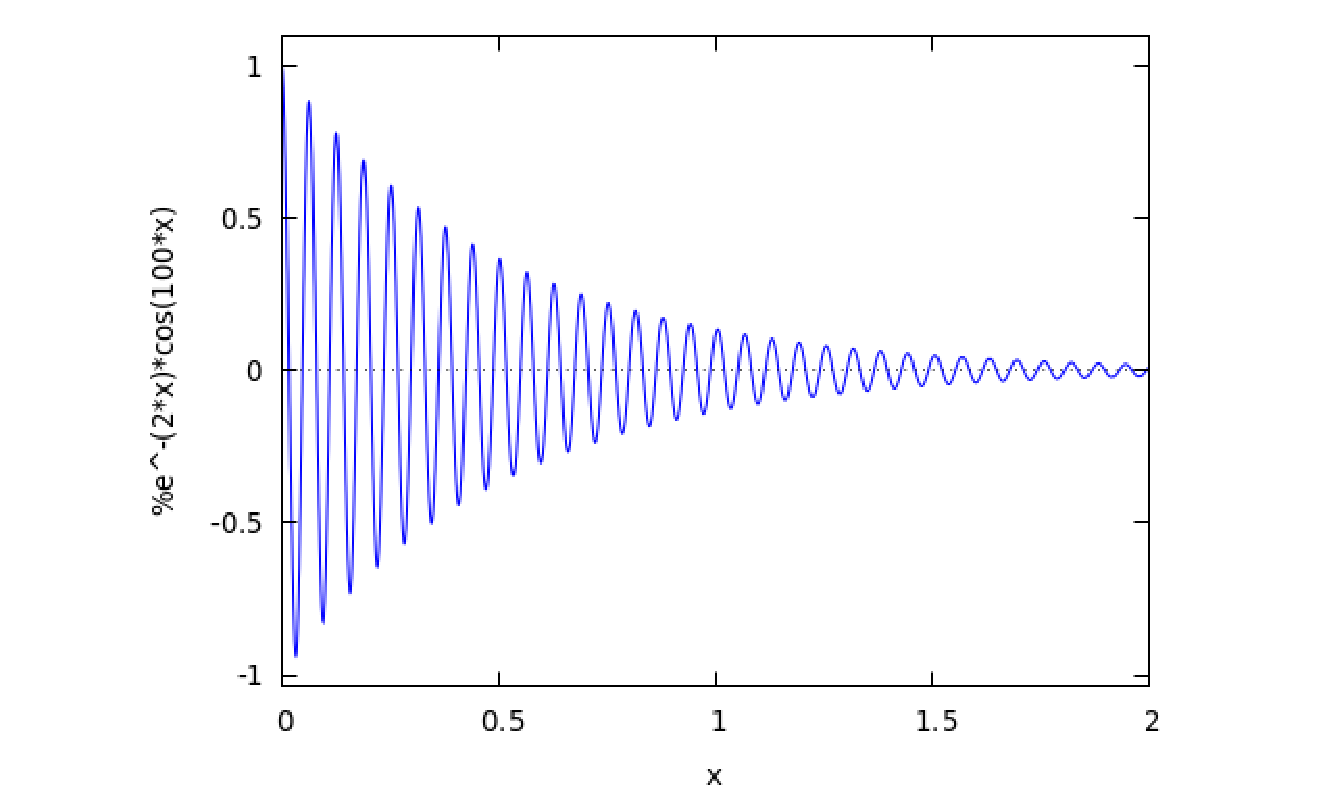
\includegraphics[width=4cm]{2022-1-C2/osc-amort.pdf}$$

\vspace*{-0.25cm}

A maioria dos livros ``normais'' de EDOs ensinam um modo de resolver a
$(*)$ que eu acho muito árido. Nesta questão você vai ver um método
pra resolver EDOs desse tipo que eu acho bem mais legal, e que eu
aprendi num curso de Álgebra Linear. Nesse método a gente trata
funções como vetores (de dimentão infinita) e a derivada como uma
transformação linear (uma ``matriz de dimensão infinita''). Quando eu
precisar enfatizar que estou ``em Álgebra Linear'' eu vou escrever $f$
e $D$ ao invés de $f(x)$ e $\ddx$.

}\anothercol{

  Isto aqui é uma demonstração quase completa do modo rápido de
  encontrar as ``soluções básicas'' e a ``solução geral'' da EDO
  $(*)$... ela é ``quase completa'' no sentido de que ela é o que as
  pessoas escrevem no quadro quando explicam esse método, mas sem a
  parte falada.
  %
  $$\scalebox{0.9}{$
    \begin{array}{rcl}
      f''(x)+7f'(x)+10f(x) &=& 0 \\
      \ddx \ddx f(x) + 7 \ddx f(x)+10f(x) &=& 0 \\
      (\ddx \ddx + 7 \ddx + 10) f(x) &=& 0 \\
      (D^2 + 7D + 10)f &=& 0 \\
      (D^2 + (2+5)D + (2·5))f &=& 0 \\
      (D+2)(D+5)f &=& 0 \\
      (D+2)(D+5)e^{-5x} &=& (D+2)(De^{-5x}+5e^{-5x}) \\
                           &=& (D+2)(-5e^{-5x}+5e^{-5x}) \\
                           &=& (D+2)0 \\
                           &=& 0 \\
      (D+5)(D+2)f &=& 0 \\
      (D+5)(D+2)e^{-2x} &=& (D+5)(De^{-2x}+2e^{-2x}) \\
                           &=& (D+5)(-2e^{-2x}+2e^{-2x}) \\
                           &=& (D+5)0 \\
                           &=& 0 \\
      (D^2 + 7D + 10)(γe^{-2x} + δe^{-5x}) &=& 0 \\
    \end{array}
    $}
    $$

    (Continua...)
}}



\newpage

% «edo-2a-ordem-cont»  (to ".edo-2a-ordem-cont")
% (c2m221p2p 6 "edo-2a-ordem-cont")
% (c2m221p2a   "edo-2a-ordem-cont")

{\bf Questão 4 (cont.)}

% «edo-2a-ordem»  (to ".edo-2a-ordem")
% (c2m221p2p 3 "edo-2a-ordem")
% (c2m221p2a   "edo-2a-ordem")
% (c2m212introp 12 "EDOs-chutar-testar")
% (c2m212introa    "EDOs-chutar-testar")


\scalebox{0.55}{\def\colwidth{10cm}\firstcol{

    ...e isto aqui é uma versão mais curta da demonstração da página
    anterior:

    $$\scalebox{0.8}{$
      \begin{array}{rcl}
        f''(x)+7f'(x)+10f(x) &=& 0 \\
        (D^2 + 7D + 10)f &=& 0 \\
        (D^2 + (2+5)D + (2·5))f &=& 0 \\
        (D^2 + 7D + 10)(γe^{-2x} + δe^{-5x}) &=& 0 \\
      \end{array}
      $}
    $$

    Aqui que você já tem uma certa prática com problemas de ``encontre
    a substituição certa'' você vai fazer um problema de ``encontre a
    generalização certa''. Vou explicar ele em português.

    \msk

    Você vai definir [EDOLP] -- de ``EDO linear, caso particular'' --
    como sendo o bloco de quatro igualdades acima. Faça isso na
    notação certa, que é algo como ``[EDOLP] = ?''.

    \msk

    Depois disso você vai procurar a ``generalização certa'' da
    [EDOLP], e na ``substituição certa'' que transforma ela na
    [EDOLP]. O seu objetivo é chegar em algo da forma [EDOLG][S] =
    [EDOLP]; o nome ``[EDOLG]'' vem de ``EDO linear, caso geral''. É
    difícil chegar na [EDOLG] direto, então vou dar instruções pra
    você chegar lá por chutar-e-testar.


}\anothercol{

  Chame as suas tentativas de [EDOLG1], [EDOLG2], etc, e as suas
  substituições de [S1], [S2], etc. O seu objetivo é chegar numa
  [EDOLG${}_n$] que não tenha mais os números 2, 5, 7 e 10; eles devem
  ter sido substuídos ou por variáveis ou por expressões que dependem
  dessas variáveis.

  \msk

  O seu objetivo {\sl final} é chegar num caso em que [S] seja só isto
  aqui:
  %
  $$\text{[S]} = \bmat{α:=2 \\ β:=5}$$

  E isto valha:
  %
  $$\text{[EDOLG]} \bmat{α:=2 \\ β:=5} \text{``=''} \text{[EDOLP]}$$

  Eu pus o \text{``=''} entre aspas porque você vai não chegar a algo
  exatamente igual à [EDOLP], só em algo equivalente à EDOLP... como o
  que a gente fez nos exercícios de ``justifique esse passo''.

  \msk

  Quem for fazer a VS vai ver como nos últimos semestres a gente usou
  essa técnica pra aprender a demonstrar algumas fórmulas das tabelas
  de integração dos livros -- a gente começava com um caso particular
  e ``generalizava ele do jeito certo'' depois.

}}




\newpage




% «links»  (to ".links")


\GenericWarning{Success:}{Success!!!}  % Used by `M-x cv'

\end{document}

%  ____  _             _         
% |  _ \(_)_   ___   _(_)_______ 
% | | | | \ \ / / | | | |_  / _ \
% | |_| | |\ V /| |_| | |/ /  __/
% |____// | \_/  \__,_|_/___\___|
%     |__/                       
%
% «djvuize»  (to ".djvuize")
% (find-LATEXgrep "grep --color -nH --null -e djvuize 2020-1*.tex")

 (eepitch-shell)
 (eepitch-kill)
 (eepitch-shell)
# (find-fline "~/2022.1-C2/")
# (find-fline "~/LATEX/2022-1-C2/")
# (find-fline "~/bin/djvuize")

cd /tmp/
for i in *.jpg; do echo f $(basename $i .jpg); done

f () { rm -v $1.pdf;  textcleaner -f 50 -o  5 $1.jpg $1.png; djvuize $1.pdf; xpdf $1.pdf }
f () { rm -v $1.pdf;  textcleaner -f 50 -o 10 $1.jpg $1.png; djvuize $1.pdf; xpdf $1.pdf }
f () { rm -v $1.pdf;  textcleaner -f 50 -o 20 $1.jpg $1.png; djvuize $1.pdf; xpdf $1.pdf }

f () { rm -fv $1.png $1.pdf; djvuize $1.pdf }
f () { rm -fv $1.png $1.pdf; djvuize WHITEBOARDOPTS="-m 1.0 -f 15" $1.pdf; xpdf $1.pdf }
f () { rm -fv $1.png $1.pdf; djvuize WHITEBOARDOPTS="-m 1.0 -f 30" $1.pdf; xpdf $1.pdf }
f () { rm -fv $1.png $1.pdf; djvuize WHITEBOARDOPTS="-m 1.0 -f 45" $1.pdf; xpdf $1.pdf }
f () { rm -fv $1.png $1.pdf; djvuize WHITEBOARDOPTS="-m 0.5" $1.pdf; xpdf $1.pdf }
f () { rm -fv $1.png $1.pdf; djvuize WHITEBOARDOPTS="-m 0.25" $1.pdf; xpdf $1.pdf }
f () { cp -fv $1.png $1.pdf       ~/2022.1-C2/
       cp -fv        $1.pdf ~/LATEX/2022-1-C2/
       cat <<%%%
% (find-latexscan-links "C2" "$1")
%%%
}

f 20201213_area_em_funcao_de_theta
f 20201213_area_em_funcao_de_x
f 20201213_area_fatias_pizza



%  __  __       _        
% |  \/  | __ _| | _____ 
% | |\/| |/ _` | |/ / _ \
% | |  | | (_| |   <  __/
% |_|  |_|\__,_|_|\_\___|
%                        
% <make>

 (eepitch-shell)
 (eepitch-kill)
 (eepitch-shell)
# (find-LATEXfile "2019planar-has-1.mk")
make -f 2019.mk STEM=2022-1-C2-P2 veryclean
make -f 2019.mk STEM=2022-1-C2-P2 pdf

% Local Variables:
% coding: utf-8-unix
% ee-tla: "c2p2"
% ee-tla: "c2m221p2"
% End:

